
\begin{figure}[ht!]
  \begin{centering}
    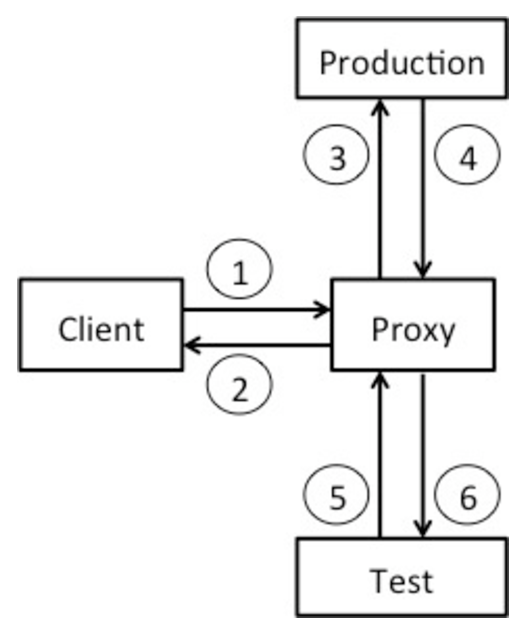
\includegraphics[width=0.4\textwidth]{figs/network_dup.eps}
    \caption{Description of the Network Duplicator. In \textit{synchronized} mode: there are 2 threads for each connection, Thread 1 executes steps [1,3,5], and Thread 2 executes [2,4,6] sequentially. In \textit{asynchronous} mode, there are 4 threads for each connection, Thread 1 executes steps [1,3], Thread 2 executes [2,4], Thread 3 executes [5], and Thread 4 executes [6]}
    \label{fig:duplicator}
  \end{centering}
\end{figure}

\subsubsection{Duplication Modes}
\label{sec:dupMode}

%\begin{enumerate}[leftmargin=*]
%\begin{enumerate}[leftmargin=*]

%\item 
\noindent
\textbf{Synchronized Packet Forwarding Mode}: 
A naive strategy is to have a single worker thread to send and receive tcp stream to the production container as well as the debug container.
%This is the simplest strategy and is quite robust as far as sending proxy data is concerned. 
To understand this better let us look at figure \ref{fig:duplicator}: Here each incoming connection would be handled by 2 parallel threads in the proxy T1, and T2. 
Where T1 sends data from the client to the proxy (communication link 1), then sends data from proxy to production (link 3), and finally from proxy to debug container (link 5). 
Whereas, thread 2 sends replies from production to proxy(link 4), then receives replies from debug container to proxy (link 6), which are then dropped. 
Thread T2 then forwards Packets received on link 4 are forwarded on link 2 to the client.

By design TCP is a connection oriented protocol and is designed for stateful delivery and acknowledgment that each packet has been delivered.
Packet sending and receiving are blocking operations by default, and hence if either the sender or the receiver is faster than the other the send/receive operations are automatically blocked or throttled.

In our case this can be viewed as follows: Let us assume that the client was sending packets at $X Mbps$ (link 1), and the production container was receiving/processing packets at $Y Mbps$ (link 3), where $Y<X$. 
Then automatically, the speed of link 1 and link 2 would be throttled to $Y Mbps$ per second, i.e the packet sending at the client would be throttled to accommodate the production server. 
Network throttling is the default TCP behavior to keep the sender and receiver synchronized.
%This behavior adheres to the default TCP protocol.
%, and if our proxy was only forwarding traffic to the production container it would be fine.
However, we also send packets to the debug-container (link 5) in the same sequential thread T1. 
Hence if the speed of link 5 is $Z$ $Mbps$, where $Z < Y$, and $Z < X$, then the speed of link 1, and link 3 would also be throttled to $Z$ $Mbps$.

%Such a communication model effects the user-experienced delay for the targeted SOA application, and is against the guiding principal of \parikshan.
The speed of the debug container is likely to be less than the production container, hence this would definetely impact the performance of the production container.
Next we discuss an asynchronous packet forwarding scheme, which avoids any slowdown to the production container.

%It especially works well with standard SOA architectures with small incoming packet flows, 
%as it means that the delay caused in the test and production container would be minimal.
%However, a major disadvantage of this approach is that every connection received would 
%finish a round trip connection with production container before sending the packets to the test-container.
%This would obviously delay all communication to the test-container by the amount of time it takes for the production container to respond. 
%However, more importantly it also effects the speed of the production container for every subsequent flow, 
%since it will have to wait for the time taken to send the packets to the test container.
%We assume a worker thread model for our proxy, where each connection is managed separately by one worker thread, 
%since our target is a service oriented architecture there should be frequent small connections from multiple users, hence a threading model is important.

%\item 
\noindent
\textbf{Asynchronous Packet Forwarding Model}: 
As shown in the previous section, in the synchronized mode the debug container, can effect the speed of the production container as well. 
The main reason for this is because of blocking sends being used to forward packets from the client to the debug-container and production container by the same sequential process.
In the asynchronous packet forwarding mode (see figure \ref{fig:duplicator}): we use 4 threads T1, T2, T3, T4 to manage each incoming connection to the proxy.
Thread T1 forwards packets from client to proxy (link 1), and from proxy to production container (link 2). 
It then uses a non-blocking send to forward packets to an internal pipe buffer shared between thread T1, and thread T3. 
Thread T3, then reads from this piped buffer and sends traffic forward to the debug-container. 
Similarly Thread T2, receives packets from production container, and forwards them to the client, while Thread T4, receives packets from the debug-container and drops them.

The advantage of this strategy is that any slowdown in the debug-container will not effect the production container's communication as a non-blocking send is used to forward traffic to the production container. 
A side-effect of this strategy is that if the speed of the debug-container is too slow compared to the production container, it may eventually lead to a buffer overflow. 
We call the time taken by a connection before which the buffer overflows is called it's \emph{debug-window}.
We discuss the implications of the \emph{debug window} in section \ref{sec:window}.  
%In this strategy we have two worker threads which simultaneously handle sending and receiving tcp streams for the production container as well as the test container.
%Whenever any event happens the connection is established, and the incoming message is read to a buffer, this buffer is then sent to a worker thread for forwarding the data to the production container, and another thread for forwarding the data to the test container. 
%This means that unlike our previous model, the processing time of either the production container or the test container will not effect the performance of the other.
%We have a slightly modified worker thread model, in which each incoming connection is managed by two worker threads one for communication with the production and the other for the test.

%\item \textbf{Asynchronous Load Balanced Packet Forwarding Model}

%It is still possible that there will be slowdown, and a short packet window because of the overhead of running test-cases in the test container. 
%This would mean that the test container will have a short time-window to execute test-cases.
To further increase this \emph{debug window}, we propose load balancing debugging across multiple debug-containers, which can each get a duplicate copy of the incoming data. 
This would mean that there are multiple threads handling the incoming connection, one for the production container, and one for each of the debug containers.
We believe that such a strategy would significantly reduce the chance of a buffer overflow in cases where the debug-container is significantly slower.

%\end{enumerate}

%The algorithm for each of the packet forwarding modes has been described in Algorithm.\ref{algoDuplication}. 
%As an added explanation, the only difference between communication with the production container v/s the test container is that the when the proxy receives the message back from the production container, it sends the stream back to the client, on the other hand for the test container the packets are simply received and then dropped.


\iffalse

Since the speed of input from the client is not in sync production-container, we need to buffer incoming traffic and relay it to the the TCP Connector(Node 6, figure \ref{fig:duplicator}) as soon as the test-container is ready for new traffic. 
Since parallel connections can be initiated by the client on the same TCP port, the Buffer-Manager creates multiple buffers for each connection, and initiates new connections by following the same causal flow of the packets received from the client. 
Unlike record-replay systems \parikshan does not claim to have strong consistency requirements, and does not need to exactly follow the production container as the goal is not reproduce all non-determinism in the production environment, but instead capture input non-determinism, and complete system state from a given point of time.
We discuss consistency requirements further in section \ref{sec:consistency}

\fi
